\documentclass{article}
\usepackage{amsmath, amssymb, bm, tikz, mathtools, tcolorbox, array, sfmath, enumerate, multicol, pgfplots}
\pgfplotsset{compat = newest}
\renewcommand{\familydefault}{\sfdefault}
\usepackage[top = 0.25in, bottom = 0.25in, left = 1in, right = 1in]{geometry}
\pagestyle{empty}
\raggedright

\newcounter{example}[section]
\newenvironment{example}[1][]{\refstepcounter{example}\par\medskip
   {\color{red}\textbf{Example~\theexample. #1}}}{\medskip}

\begin{document}

\section*{Domain and Range}

\begin{tcolorbox}[colframe=orange!70!white, coltitle=black, title=\textbf{Summary}]
\begin{enumerate}
    \item Domain: all possible input; Range: all possible output.
\end{enumerate}
\end{tcolorbox}

\subsection*{Domain (Visual)} \vspace{11pt}

The \textbf{domain} of a function is the set of all possible inputs (usually $x$) of the function. \newline

In other words, \textbf{domain} is all possible $x$-coordinates on the function's graph. \newline

\begin{example}Determine the domain of each. Write your answer as an inequality or a compound inequality.
\end{example}

\begin{enumerate}[(a)]
\begin{multicols}{2}
\item \mbox{} \newline\\ 
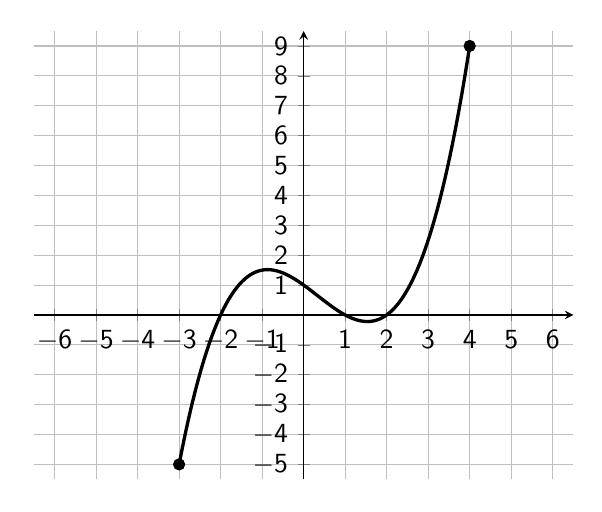
\begin{tikzpicture}
\begin{axis}
[axis lines = middle, xmin = -6.5, xmax = 6.5, ymin = -5.5, ymax = 9.5, grid, xtick distance = 1, ytick distance = 1]
\addplot[very thick, domain=-3:4, samples=200] plot {0.25*(x+2)*(x-1)*(x-2)};
\addplot[mark = *, only marks] coordinates {(-3,-5) (4,9)};
\end{axis}
\end{tikzpicture}
\item \mbox{} \newline\\ 
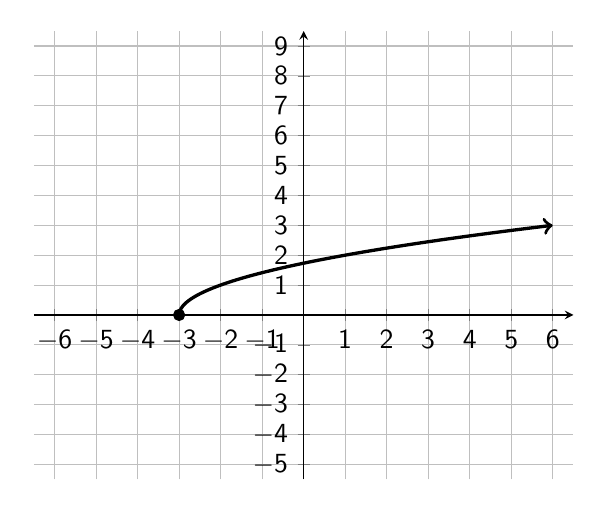
\begin{tikzpicture}
\begin{axis}
[axis lines = middle, xmin = -6.5, xmax = 6.5, ymin = -5.5, ymax = 9.5, grid, xtick distance = 1, ytick distance = 1]
\addplot[->, very thick, domain=-3:6, samples=200] plot {sqrt(x+3)};
\addplot[mark = *, only marks] coordinates {(-3,0)};
\end{axis}
\end{tikzpicture}
\end{multicols}

\vspace{0.5in}

\begin{multicols}{2}
\item \mbox{} \newline\\ 
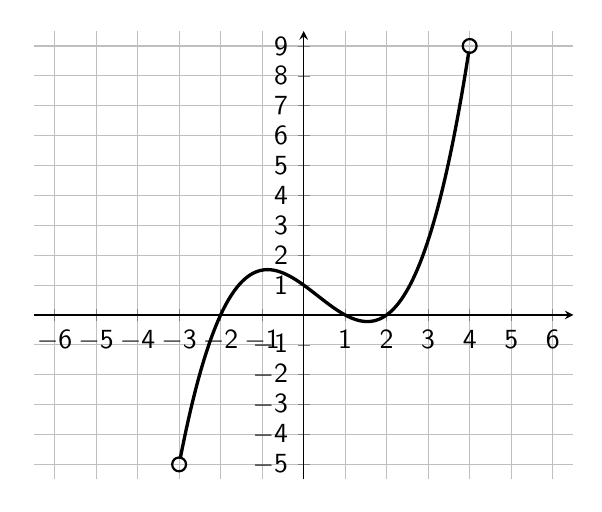
\begin{tikzpicture}
\begin{axis}
[axis lines = middle, xmin = -6.5, xmax = 6.5, ymin = -5.5, ymax = 9.5, grid, xtick distance = 1, ytick distance = 1]
\addplot[very thick, domain=-3:4, samples=200, shorten <= 2pt, shorten >= 2pt] plot {0.25*(x+2)*(x-1)*(x-2)};
\addplot[thick, mark = o, only marks, mark options={scale=1.25}] coordinates {(-3,-5) (4,9)};
\end{axis}
\end{tikzpicture}
\item \mbox{} \newline\\ 
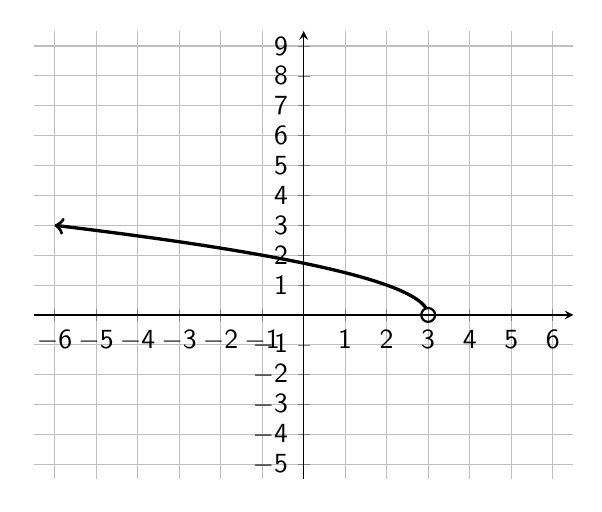
\begin{tikzpicture}
\begin{axis}
[axis lines = middle, xmin = -6.5, xmax = 6.5, ymin = -5.5, ymax = 9.5, grid, xtick distance = 1, ytick distance = 1]
\addplot[<-, very thick, domain=-6:2.95, samples=200] plot {sqrt(-x+3)};
\addplot[thick, mark = o, only marks, mark options={scale=1.25}] coordinates {(3,0)};
\end{axis}
\end{tikzpicture}
\end{multicols}
\end{enumerate}

\newpage 

\subsection*{Domain (Equations)} \vspace{11pt}

For most of the functions in this section of the notes, the domain will be {\color{red}\textbf{all real numbers}}.
\bigskip 

However, there are {\color{violet}\textbf{2 exceptions:}}
\begin{enumerate}
    \item Functions with a variable in the denominator: \quad denominator $\neq$ 0
    \item Functions inside a square root: \quad $\sqrt{\geq 0}$
\end{enumerate}
\bigskip 

\begin{example}
State the domain of each.
\begin{multicols}{3}
\begin{enumerate}[(a)]
    \item $f(x) = 3x - 2$
    \item $g(x) = 6x^2 + 4$
    \item $h(x) = \sqrt{x-7}$
\end{enumerate}
\end{multicols}
\vfill 
\begin{multicols}{3}
\begin{enumerate}[(a)]  \setcounter{enumi}{3}
    \item $j(x) = \sqrt{2x+4}$
    \item $m(x) = \frac{5}{x-2}$
    \item $p(x) = \frac{3}{x+9}$
\end{enumerate}
\end{multicols}
\end{example}
\vfill

\newpage 

\subsection*{Range (Visual)} \vspace{11pt}

The \textbf{range} of a function is the set of all possible outputs (usually $y$) of the function. \newline

In other words, \textbf{range} is all possible $y$-coordinates on the function's graph. \newline

\begin{example}
Determine the range of each. Write your answer as an inequality or a compound inequality. \end{example}

\begin{enumerate}[(a)]
\begin{multicols}{2}
\item \mbox{} \newline\\ 
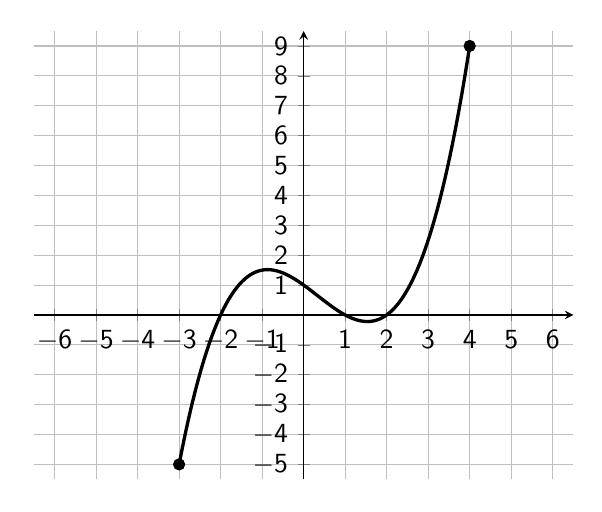
\begin{tikzpicture}
\begin{axis}
[axis lines = middle, xmin = -6.5, xmax = 6.5, ymin = -5.5, ymax = 9.5, grid, xtick distance = 1, ytick distance = 1]
\addplot[very thick, domain=-3:4, samples=200] plot {0.25*(x+2)*(x-1)*(x-2)};
\addplot[mark = *, only marks] coordinates {(-3,-5) (4,9)};
\end{axis}
\end{tikzpicture}
\item \mbox{} \newline\\ 
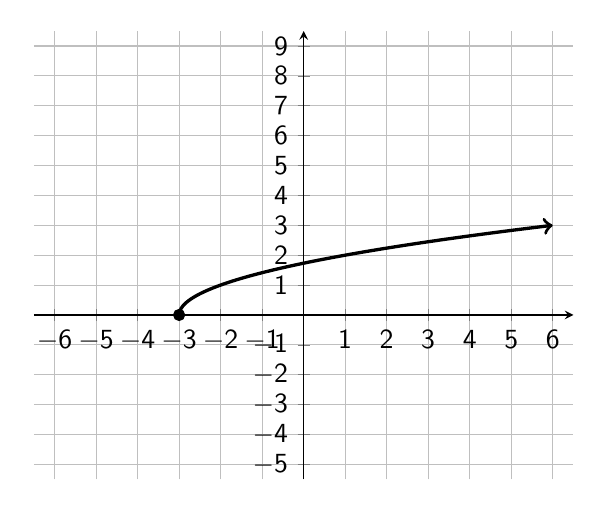
\begin{tikzpicture}
\begin{axis}
[axis lines = middle, xmin = -6.5, xmax = 6.5, ymin = -5.5, ymax = 9.5, grid, xtick distance = 1, ytick distance = 1]
\addplot[->, very thick, domain=-3:6, samples=200] plot {sqrt(x+3)};
\addplot[mark = *, only marks] coordinates {(-3,0)};
\end{axis}
\end{tikzpicture}
\end{multicols}

\vspace{0.5in}

\begin{multicols}{2}
\item \mbox{} \newline\\ 
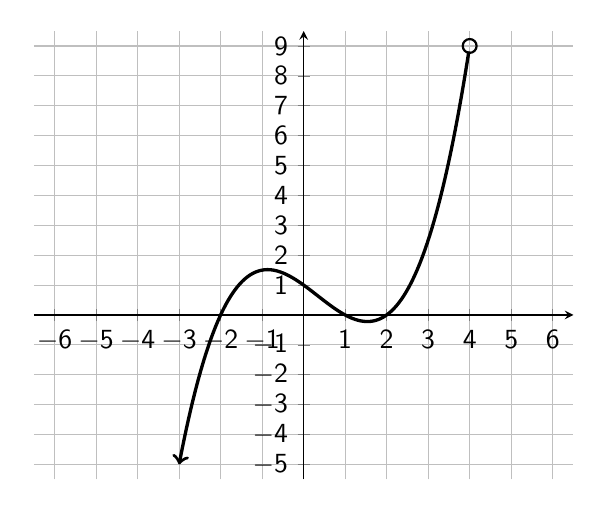
\begin{tikzpicture}
\begin{axis}
[axis lines = middle, xmin = -6.5, xmax = 6.5, ymin = -5.5, ymax = 9.5, grid, xtick distance = 1, ytick distance = 1]
\addplot[<-, very thick, domain=-3:4, samples=200, shorten >= 2pt] plot {0.25*(x+2)*(x-1)*(x-2)};
\addplot[thick, mark = o, only marks, mark options={scale=1.25}] coordinates {(4,9)};
\end{axis}
\end{tikzpicture}
\item \mbox{} \newline\\ 
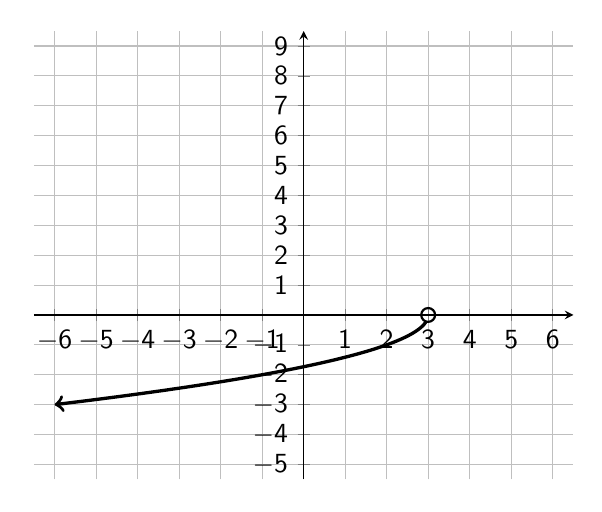
\begin{tikzpicture}
\begin{axis}
[axis lines = middle, xmin = -6.5, xmax = 6.5, ymin = -5.5, ymax = 9.5, grid, xtick distance = 1, ytick distance = 1]
\addplot[<-, very thick, domain=-6:2.95, samples=200] plot {-sqrt(-x+3)};
\addplot[thick, mark = o, only marks, mark options={scale=1.25}] coordinates {(3,0)};
\end{axis}
\end{tikzpicture}
\end{multicols}
\end{enumerate}

\end{document}
